\chapter{Basics}
\section{Definitions}
\begin{itemize}
\item A Graph is a set of objects and the relationships between pairs of objects
\item A Graph $G(V,E)$, is a set of V \textbf{Vertices/nodes} and $E$ \textbf{Edges}
\end{itemize}
\begin{figure}[h]
	\centering
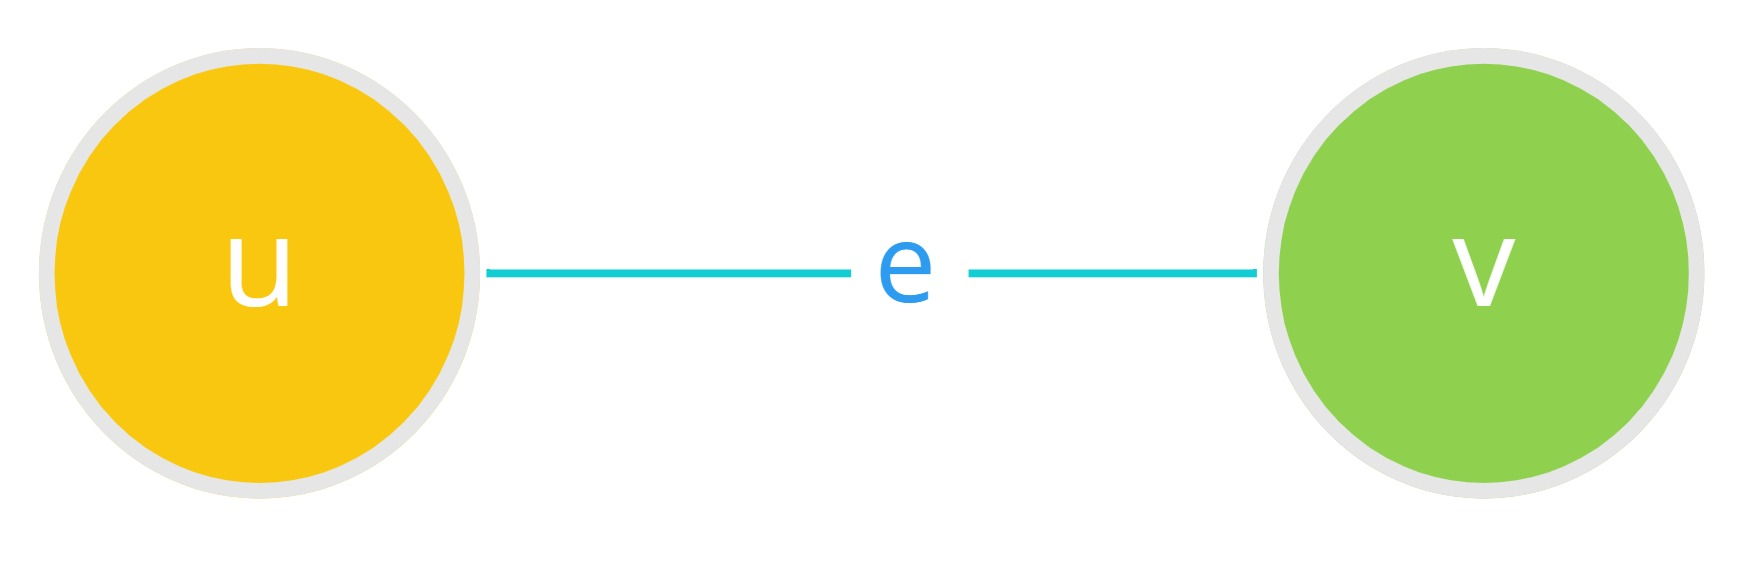
\includegraphics[scale = 0.1]{1.png}
\caption{A visual representation of a simple Graph}
\end{figure}
\begin{itemize}
\item For the above figure we say that:
\begin{itemize}
\item $e$ \textbf{Connects} $u$ and $v$
\item $u$ and $v$ are \textbf{End Points} of $e$
\item $u$ and $e$ are \textbf{Incident}
\item $u$ and $v$ are \textbf{Adjacent}
\item $u$ and $v$ are \textbf{Neighbors}
\end{itemize}
\item Or in set theory lingo as $G(\{u,v\},\{e\})$
\end{itemize}
\begin{figure}[h]\label{fig_2}
	\centering
	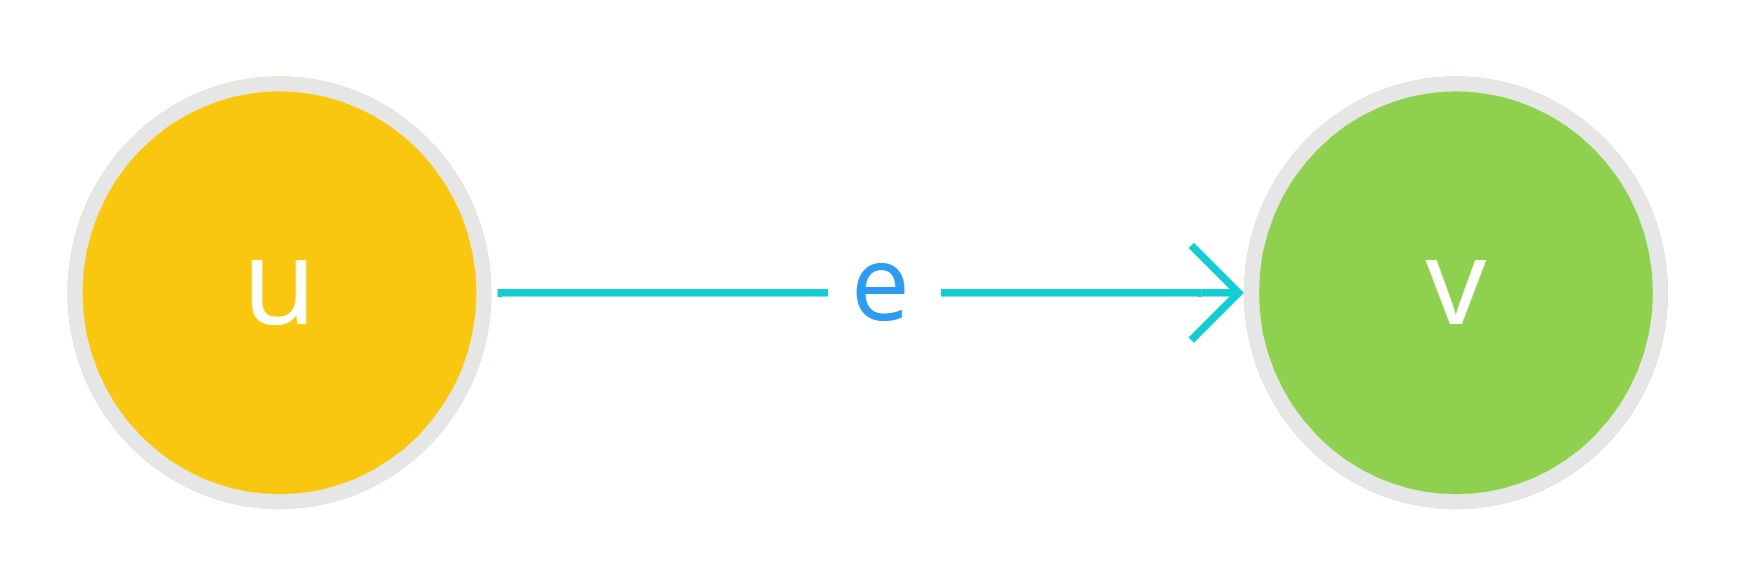
\includegraphics[scale = 0.1]{2.png}
	\caption{A visual representation of a simple directed Graph. Here $u$ is called the \textbf{tail} and $v$ the \textbf{head}}
\end{figure}
\begin{itemize}
\item There also exist \textbf{directed Edges/Arcs} i.e. , they describe asymmetric relations
\item Adding \ref{fig_2} to another directed graph with the same vertices but the edge pointing in the other direction results in a non-directed graph
\item \textbf{Degree} of a vertex is the number of its incident edges i.e. neighbours denoted by $deg(v)$
\item The degree of a graph is the maximum degree of its vertices
\end{itemize}
\section{Types of Graph}
\begin{itemize}
\item A \textbf{Regular graph} is a graph where each vertex has the same degree
\item A regular graph of $n$ degrees is called $n-$Regular
\item  The Complement of a graph $G = (V, E)$ is a graph $\bar{G} = (V, \bar{E})$ on the same set of vertices $V$ and the following set of edges:
\begin{itemize}
\item Two vertices are connected in $\bar{G}$ $\ iff$ they are not connected in $G$ i.e. $(u,v) \in \bar{E} \ iff \  (u,v) \notin E$
\item A \textbf{Path} is a continuous sequence of edges that connect two vertices
\item A \textbf{Walk} in a graph is a sequence of edges, such that each edge except for the first one starts with a vertex where the previous edge ended
\item The \textbf{Length} of a walk is the number of edges in it
\item A \textbf{Path} (rigorously) is a walk where all edges are distinct
\item A \textbf{Simple Path} is a walk where all vertices are distinct
\end{itemize}
\item  A \textbf{Cycle} in a graph is a path whose first vertex is the same as the last one; In particular, \textit{all the edges in a Cycle are
	distinct}
\item A \textbf{Simple Cycle} is a cycle where all vertices
except for the first one are distinct and
there first vertex is taken twice
\item A graph is called \textbf{Connected} if there is a path
between every pair of its vertices
\item  A \textbf{Connected Component} of a graph $G$ is a
maximal connected subgraph of $G$ i.e., a connected subgraph of $G$ which is not
contained in a larger connected subgraph of $G$
\item The \textbf{Indegree} of a vertex $v$ is the number of
edges ending at $v$
\item The \textbf{Outdegree} of a vertex $v$ is the number of
edges leaving $v$
\item A \textbf{Weighted Graph} associates a \textit{weight} with
every edge
\item The \textbf{Weight} of a path is the sum of the
weights of its edges
\item A \textbf{Shortest Path} between two vertices is a
path of the minimum weight
\item The \textbf{Distance} between two vertices is the
length of a shortest path between them
\end{itemize}
\begin{itemize}
\item A \textbf{Path Graph} $P_{n} \ \forall \ n \geq 2$, has $n$ vertices labeled $v_{n}$ and $n-1$ edges $\{v_{n-1}, v_{n}\}$
\end{itemize}
\begin{figure}[h]\label{fig_3}
	\centering
	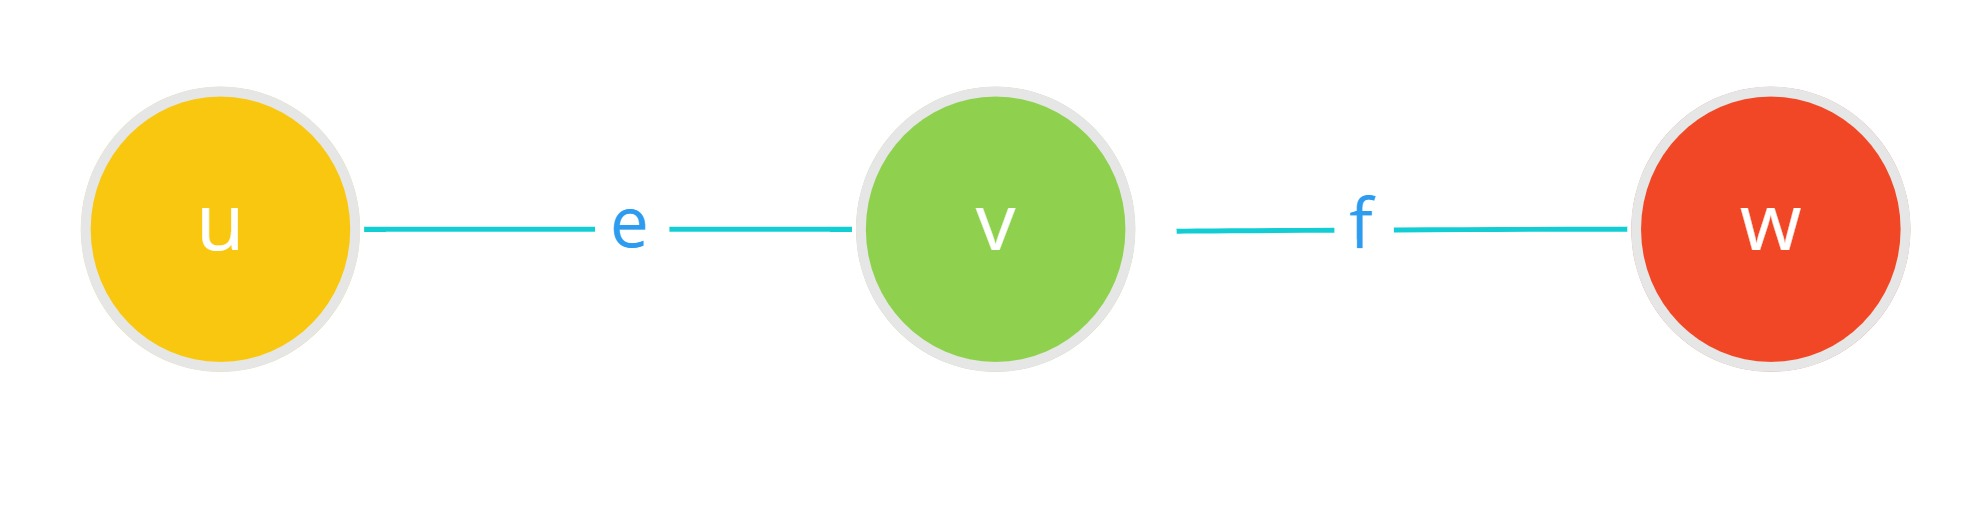
\includegraphics[scale = 0.1]{3.png}
	\caption{The Path Graph $P_{3}$}
\end{figure}
\begin{itemize}
\item A \textbf{Cycle Graph} $C_{n} \ \forall \ n \geq 3$, has $n$ vertices labeled $v_{n}$ and $n$ edges $\{v_{n-1}, v_{n}\},\{v_{n}, v_{1}\}$
\end{itemize}
\begin{figure}[h]\label{fig_4}
	\centering
	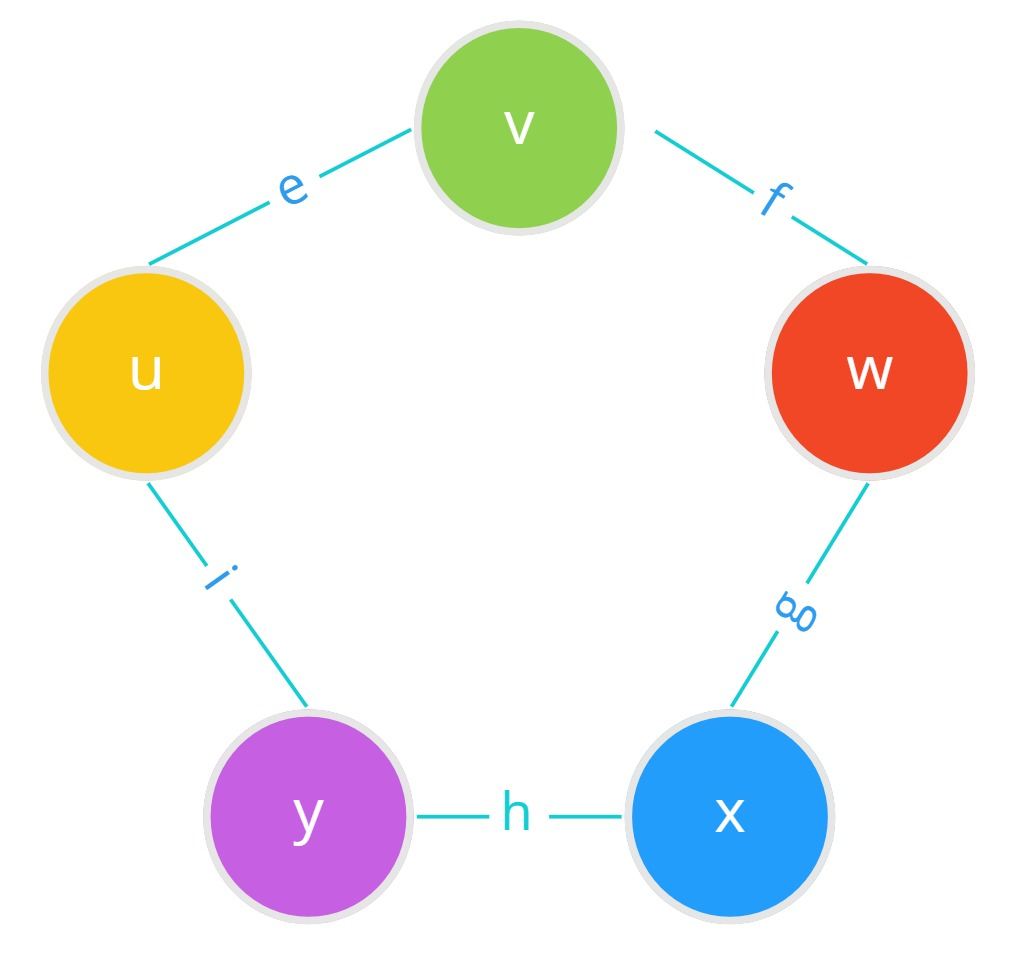
\includegraphics[scale = 0.1]{4.png}
	\caption{The Cycle Graph $C_{5}$}
\end{figure}
\pagebreak
\begin{itemize}
	\item A \textbf{Complete Graph (a.k.a Clique)} $K_{n} \ \forall \ n \geq 2$, has $n$ vertices labeled $v_{n}$ and all edges between them (i.e. $n(n-1)/2$ edges )
\end{itemize}
\begin{figure}[h]\label{fig_5}
	\centering
	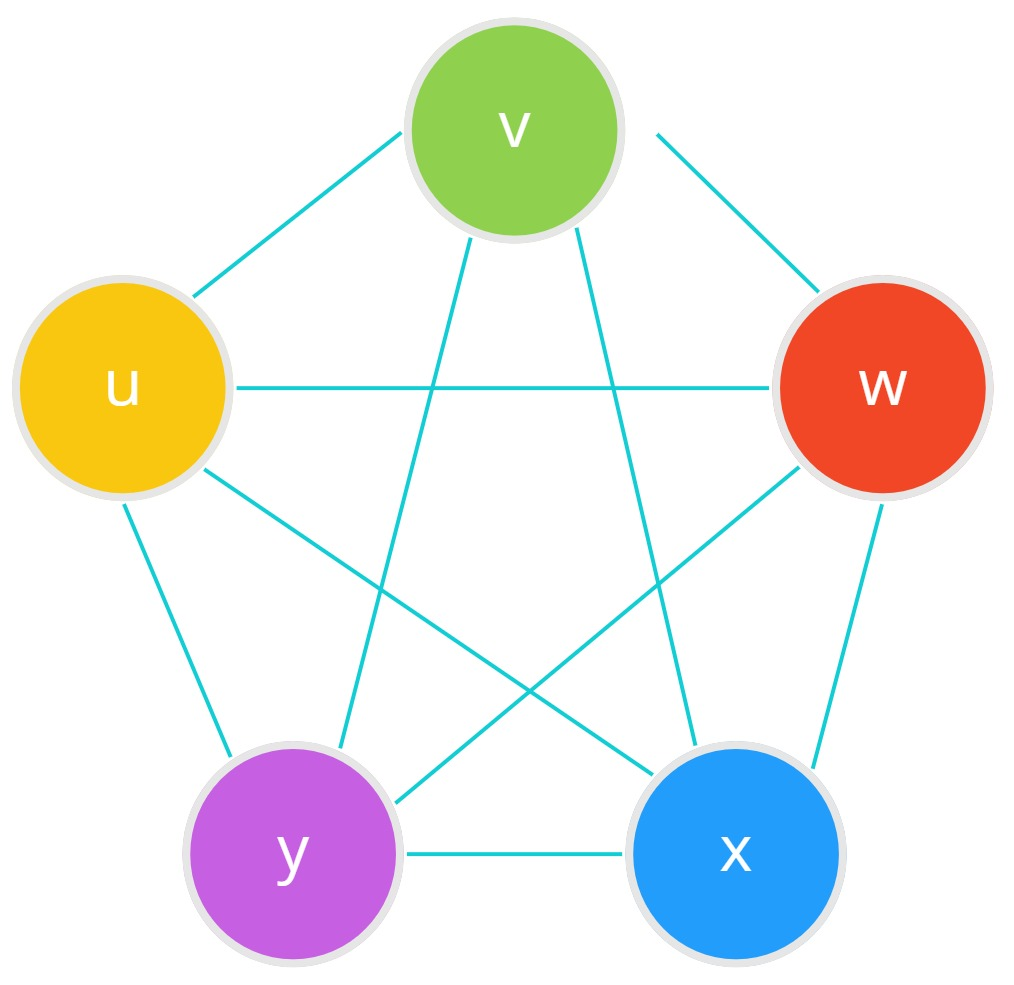
\includegraphics[scale = 0.1]{5.png}
	\caption{The Clique Graph $K_{5}$}
\end{figure}
\section{Trees}
\begin{itemize}
\item A tree is a connected graph without cycles
\item A tree is a connected graph on $n$ vertices with $n - 1$ edges
\item A graph is a tree if and only if there is a unique simple path between any pair of its vertices
\end{itemize}
\begin{figure}[h]\label{fig_2}
	\centering
	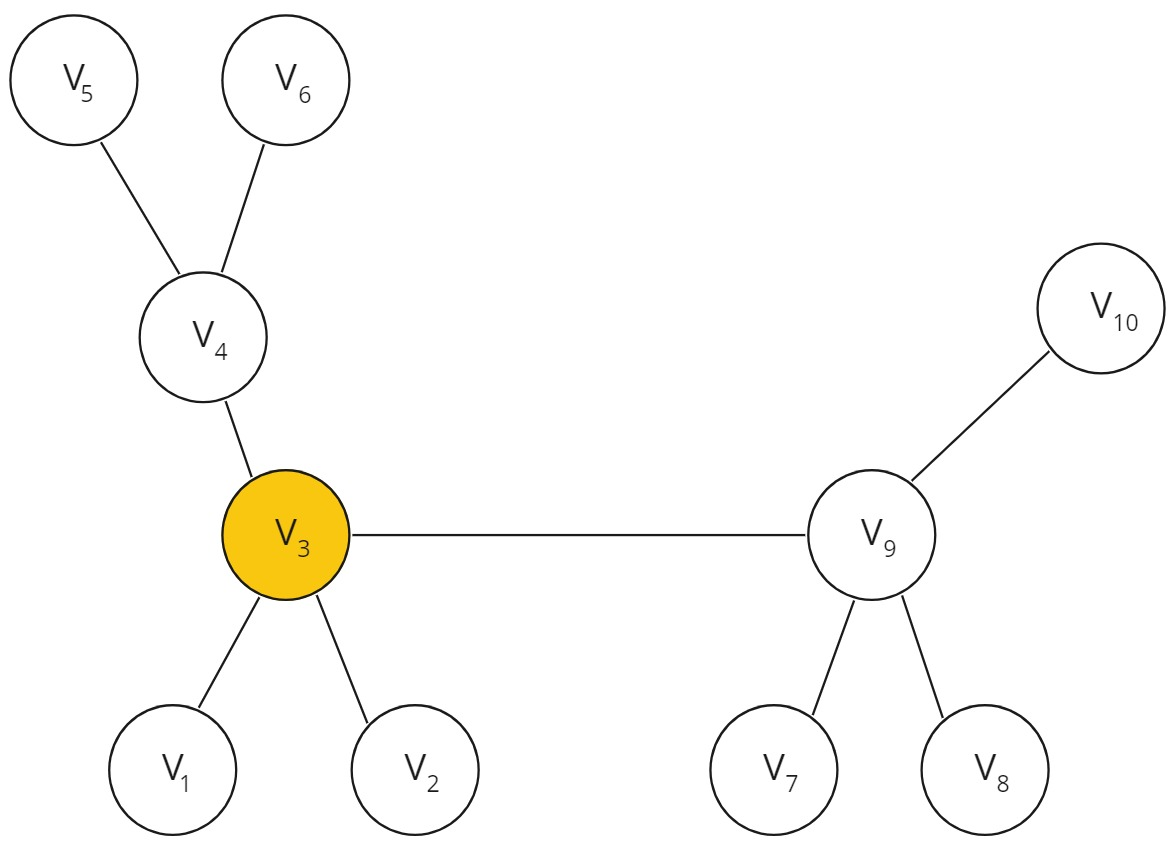
\includegraphics[scale = 0.15]{6.png}
	\caption{$C_{5}$ is not bipartite. In general, for odd $n > 2$, $C_{n}$ is not bipartite. However, }
\end{figure}
\begin{figure}[h]\label{fig_2}
	\centering
	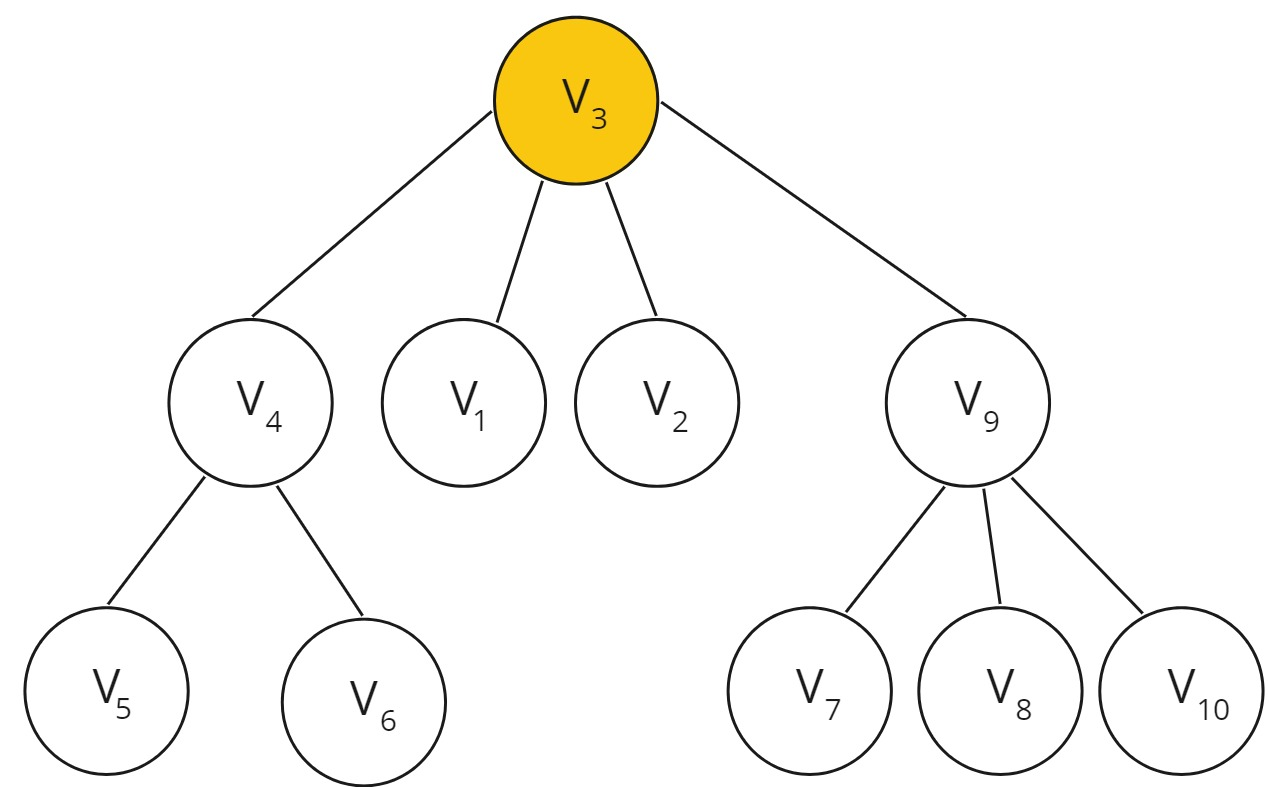
\includegraphics[scale = 0.15]{7.png}
	\caption{$C_{5}$ is not bipartite. In general, for odd $n > 2$, $C_{n}$ is not bipartite. However, }
\end{figure}
\subsection{How to make a tree?}
\begin{itemize}
\item Remove any edge, keeping the Graph connected
\end{itemize}
\begin{figure}[h]\label{fig_5}
	\centering
	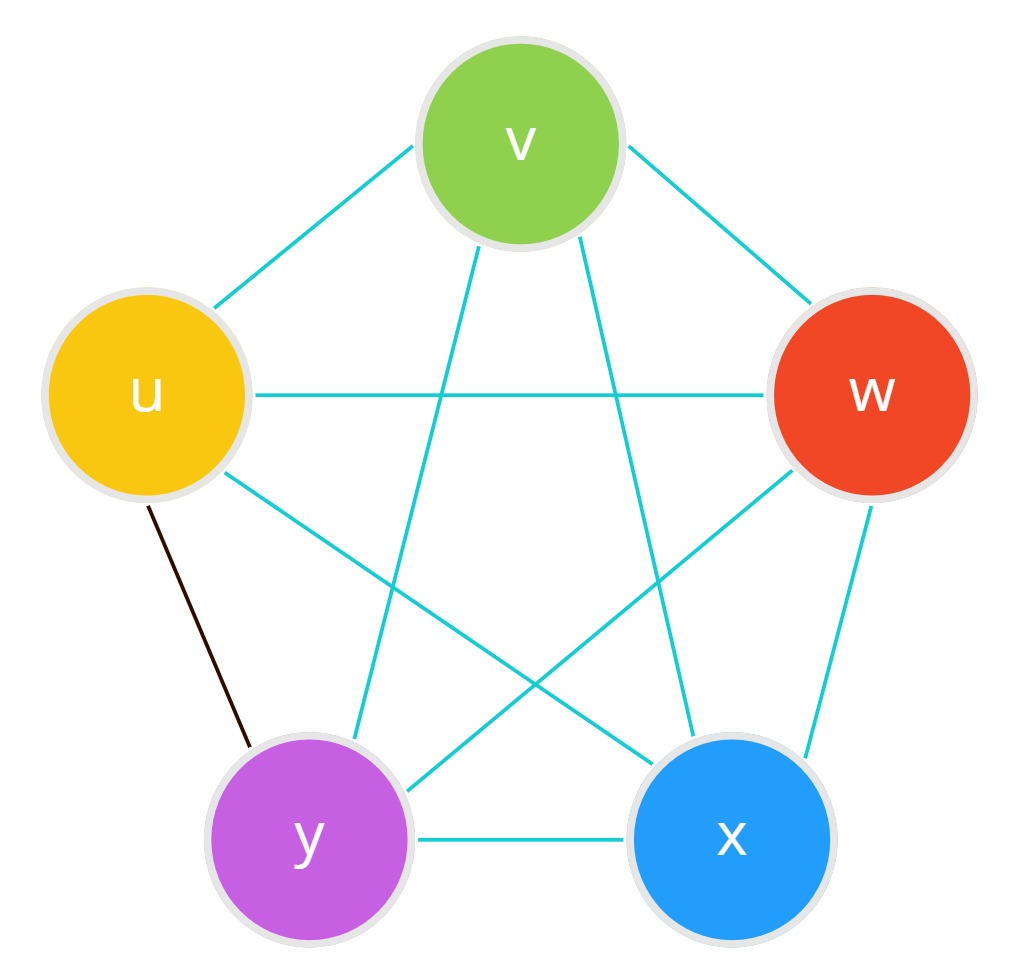
\includegraphics[scale = 0.1]{8.1.png}
\end{figure}
\begin{itemize}
\item Stop only when $n-1$ edges are left
\end{itemize}
\begin{figure}[h]\label{fig_5}
	\centering
	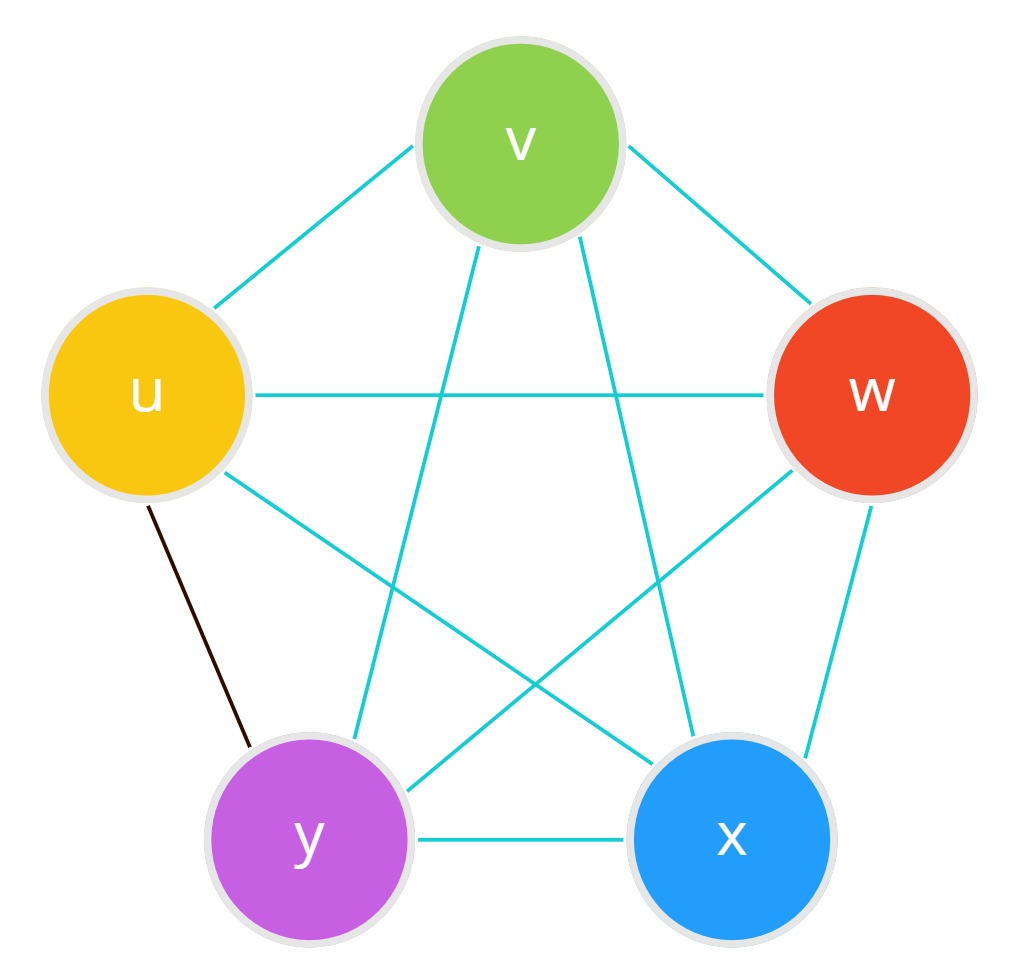
\includegraphics[scale = 0.1]{8.1.png}
\end{figure}
\section{Bipartite Graphs}
\begin{itemize}
\item A graph $G$ is \textbf{Bipartite} if its vertices can be partitioned into two disjoint sets (sets with no common elements) $L$ and $R$ such that every edge of $G$ connects a vertex in $L$ to a vertex in $R$  i.e., no edge connects two vertices from
the same part
\item $L$ and $R$ are called the parts of $G$
\item Trees are Bipartite Graphs
\begin{figure}[h]\label{fig_2}
	\centering
	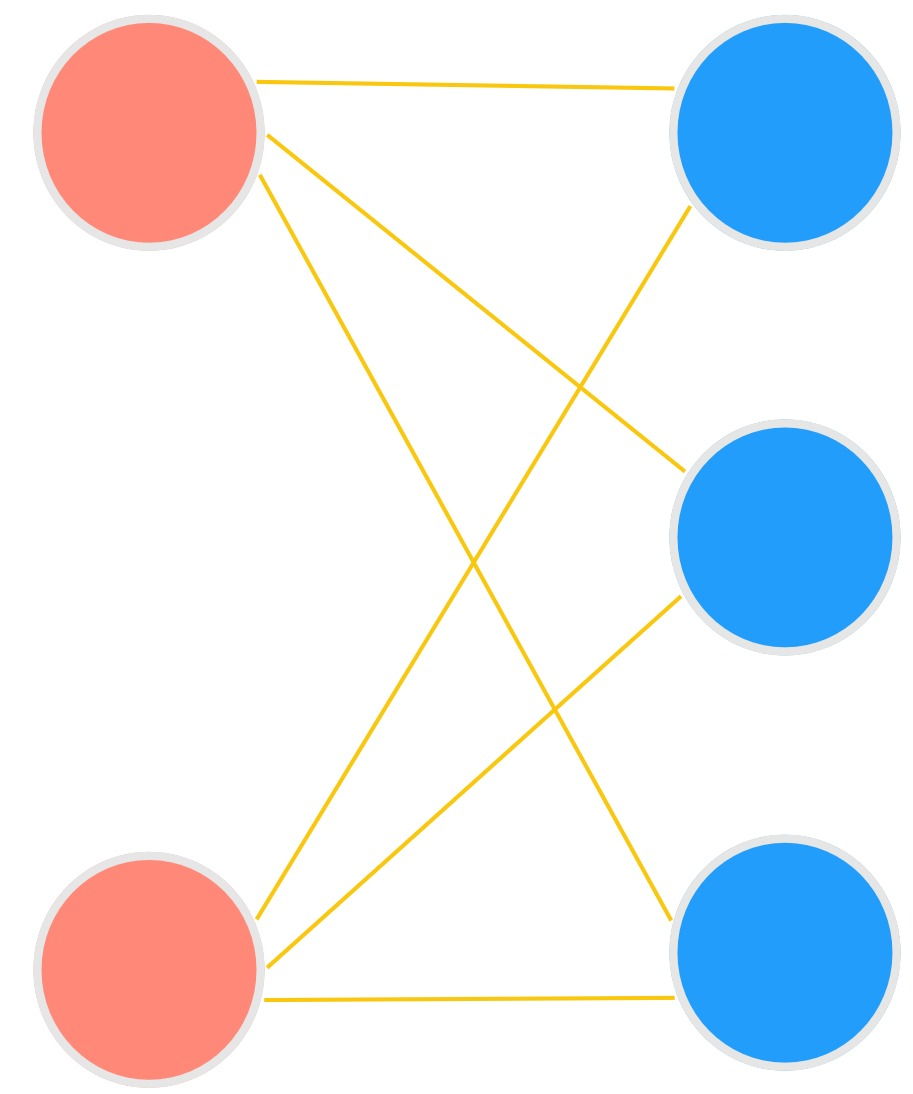
\includegraphics[scale = 0.1]{9.png}
	\caption{$C_{5}$ is not bipartite. In general, for odd $n > 2$, $C_{n}$ is not bipartite. However, }
\end{figure}
\end{itemize}
\subsection{Examples and counter examples}
\begin{figure}[h]\label{fig_2}
	\centering
	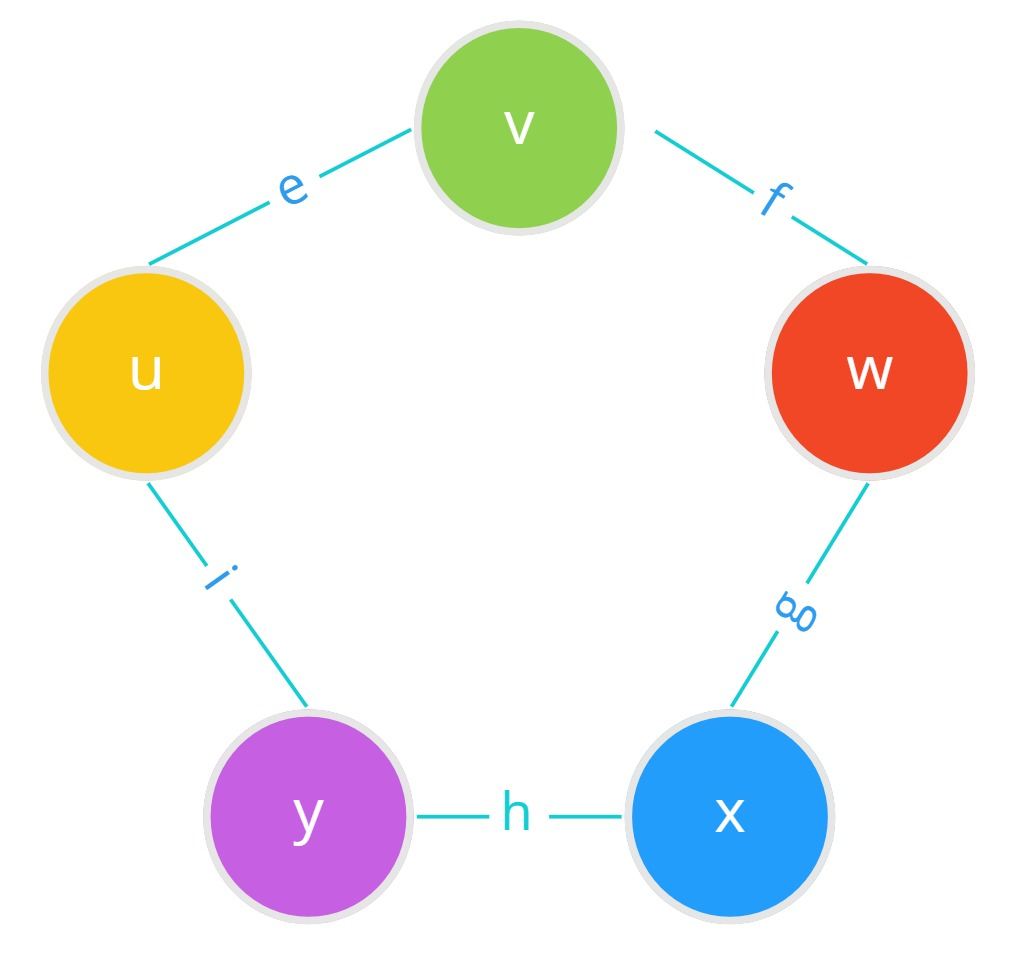
\includegraphics[scale = 0.1]{4.png}
	\caption{$K_{2,3}$ is bipartite}
\end{figure}
